\documentclass{article}

\usepackage{a4wide}
\usepackage[utf8]{inputenc}
\usepackage[T1]{fontenc}
\usepackage[french]{babel}
\usepackage[babel=true]{csquotes} 
\usepackage{graphicx}
\graphicspath{{Images/}}
\usepackage{color}
\usepackage{hyperref}
\hypersetup{colorlinks,linkcolor=,urlcolor=blue}

\usepackage{amsmath}
\usepackage{amssymb}

\title{D\'{e}veloppement pour mobiles 2 \\ MASTERMIND : Unlimited Edition }
\author{GASTELLIER Alison et BOYER Luis \\ L3 Informatique}
\date{2018}

\begin{document}
\maketitle

\begin{abstract}
Ce document est un rapport concernant le projet donn\'{e} au cours de l'Unit\'{e} d'enseignement D\'{e}veloppement pour mobiles 2. Ce projet avait pour objectif la cr\'{e}ation du m\^{e}me jeu sous iOs et Android avec un certain nombres de contraintes. On y d\'{e}crira donc toutes les \'{e}tapes importantes de sa conception.
\end{abstract}

\bigskip
\bigskip
\section{Introduction}

D'apr\`{e}s les derni\`{e}res \'{e}tudes effectu\'{e}es sur les parts du march\'{e} concernant les syst\`{e}mes d'exploitations ( OS ) utilis\'{e}s par les mobiles, Android et iOS occupent 99.6\% du march\'{e}. La quasi totalit\'{e} des mobiles utilisant donc ces OS, il est important pour un d\'{e}veloppeur de pouvoir cr\'{e}er des applications utilisables par ces deux derniers. L'Unit\'{e} d'enseignement D\'{e}veloppement pour mobiles 2 a \'{e}t\'{e} pour nous l'occasion de les rencontrer et de pouvoir nous essayer au d\'{e}veloppement d'une application qui devrait fonctionner sur Androit et iOS.
\\ \indent L'objectif \'{e}tait de cr\'{e}er un jeu comportant les contraintes suivantes : un score doit \^{e}tre associ\'{e} \`{a} chaque partie, possibilit\'{e} de sauvegarder une partie et son score, fonctionne sur tout type d'\'{e}cran en mode portrait et paysage. 
\\ \indent Le jeu que nous avons d\'{e}cid\'{e} de cr\'{e}er est une reprise du c\'{e}l\`{e}bre jeu MasterMind. Nous allons par la suite commencer par vous pr\'{e}senter les principes de notre jeu. Puis nous d\'{e}crirons l'interface sous les deux plateformes. Apr\`{e}s, nous soulignerons quelques particularit\'{e}s du code. Enfin, nous parlerons du syst\`{e}me de sauvegarde que nous avons mis en place. Nous conclurons \`{a} la fin sur le r\'{e}sultat obtenu et sur les am\'{e}liorations possibles de l'application.


\section{Principes}

MASTERMIND : Unlimited Edition reprend les principes du jeu MasterMind, avec une l\'{e}g\`{e}re variante qui est l'ajout d'un score associ\'{e} \`{a} chaque partie afin de respecter les contraintes impos\'{e}es. Le joueur devra donc essayer de deviner une combinaison de quatre couleurs choisies al\'{e}atoirement parmi six couleurs diff\'{e}rentes. Pour l'aider, deux couleurs suppl\'{e}mentaires appara\^{i}tront \`{a} c\^{o}t\'{e} de chacun de ses essais pour lui indiquer le nombre de bonnes couleurs et si ces derniers sont plac\'{e}es ou non au bon endroit. Le but du joueur est donc d'essayer \`{a} chaque partie de battre ses pr\'{e}c\'{e}dents scores.
\bigskip
\section{Interface}

L'id\'{e}e \'{e}tait d'offrir \`{a} l'utilisateur suffisamment d'essais pour rendre le jeu accessible tout en gardant une interface claire. Nous avons d\'{e}cid\'{e} que l'interface finale comporterait donc :
	 \\ - 12 lignes pour 12 essais pour l'utilisateur, 
	 \\ - un bouton " VALIDER " pour valider son essai et la comparer \`{a} la solution, 
	 \\ - un bouton " ? " pour rappeler \`{a} l'utilisateur les r\`{e}gles du jeu,
	 \\ - un bouton " QUITTER " afin de pouvoir quitter la partie en cours,
	 \\ - un label " SCORE " pour rappeler \`{a} l'utilisateur son nombre de points,
	 \\ - un bouton " SOLUTION " afin de laisser \`{a} l'utilisateur la possibilit\'{e} d'abandonner et de voir la combinaison gagnante avant de passer sur l'\'{e}cran suivant.

\subsection{Android}
Sous Android, il est très facile de gérer les tailles et orientations d'écran, il suffit de créer un \textit{Layout} réservé soit à la taille de l'écran, soit sa position. 
\begin{center}
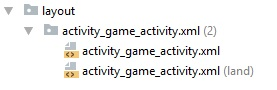
\includegraphics{layout}
\end{center}
On obtient les résultats suivants :
\begin{center}
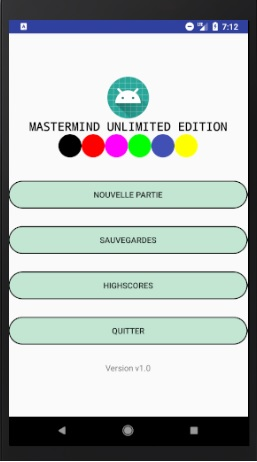
\includegraphics[scale = 0.5]{Menu} 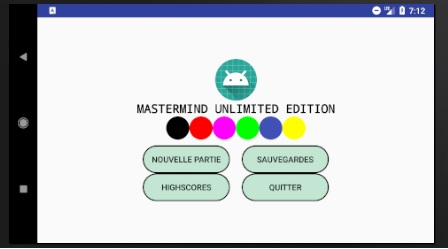
\includegraphics[scale = 0.5]{Menu_land}
\end{center}
Notre application étant assez simple au niveau graphique, nous n'avons pas eu besoin de traiter chaque taille d'écran disponibles. La gestion des  conteneurs \textit{Layout} sont suffisants pour bien présenter sous tout téléphone.


\subsection{iOS}

Sous iOS, il ne nous \'{e}tait pas offert la possibilit\'{e} de pouvoir g\'{e}rer la partie portrait et paysage s\'{e}par\'{e}ment et en fonction de tous les \'{e}crans. Il fallait donc apporter des contraintes graphiques sur chaque \'{e}l\'{e}ment ( boutons, textes, ... ) afin qu'ils gardent une certaine proportion par rapport \`{a} l'appareil sur lequel l'application \'{e}tait lanc\'{e}e. Effectivement, ayant pour objectif de pouvoir jouer avec des cercles afin de rester le plus proche possible du jeu de soci\'{e}t\'{e}, il fallait sous iOS utiliser des carr\'{e}s pour pouvoir ensuite transformer ces derniers en cercle. Cependant, nous nous sommes rendus compte plus tard qu'il n'\'{e}tait pas possible de garder des carr\'{e}s en mode paysage et portrait et ce sur tous les appareils en m\^{e}me temps. Nous avons donc opt\'{e} pour une solution offerte par l'Interface Builder de Xcode dans le Size Inspector : Autoresizing. En cochant les fl\`{e}ches comme on peut le voir ci-dessous, l'\'{e}l\'{e}ment graphique concern\'{e} gardera automatiquement une certaine proportion sembable sur tous les \'{e}crans par rapport \`{a} la proportion qu'a cet \'{e}l\'{e}ment sur l'\'{e}cran actuel. Nous pouvions alors obtenir des carr\'{e}s plus ou moins parfaits.
\begin{center}

\includegraphics{Autoresizing}
\end{center}

\indent Une fois ces carr\'{e}s obtenus nous nous attaquions donc \`{a} la transformation de ces carr\'{e}s en cercle en utilisant la propri\'{e}t\'{e} \textit{cornerRadius} des boutons. Afin de faire d'un carr\'{e} un cercle il faut donner comme valeur \`{a} cette propri\'{e}t\'{e} la moiti\'{e} de la valeur de la largeur du carr\'{e} concern\'{e}. Malheureusement, au travers des diff\'{e}rents test effectu\'{e}s nous avons pu observer qu'en dessous d'une certaine taille, on obtenait un oval et non un cercle. Pour garder une certaine homog\'{e}n\'{e}it\'{e} nous avons donc gard\'{e} des carr\'{e}s sous l'interface iOS. 
Voil\`{a} ce \`{a} quoi elle ressemble : 
\begin{center}
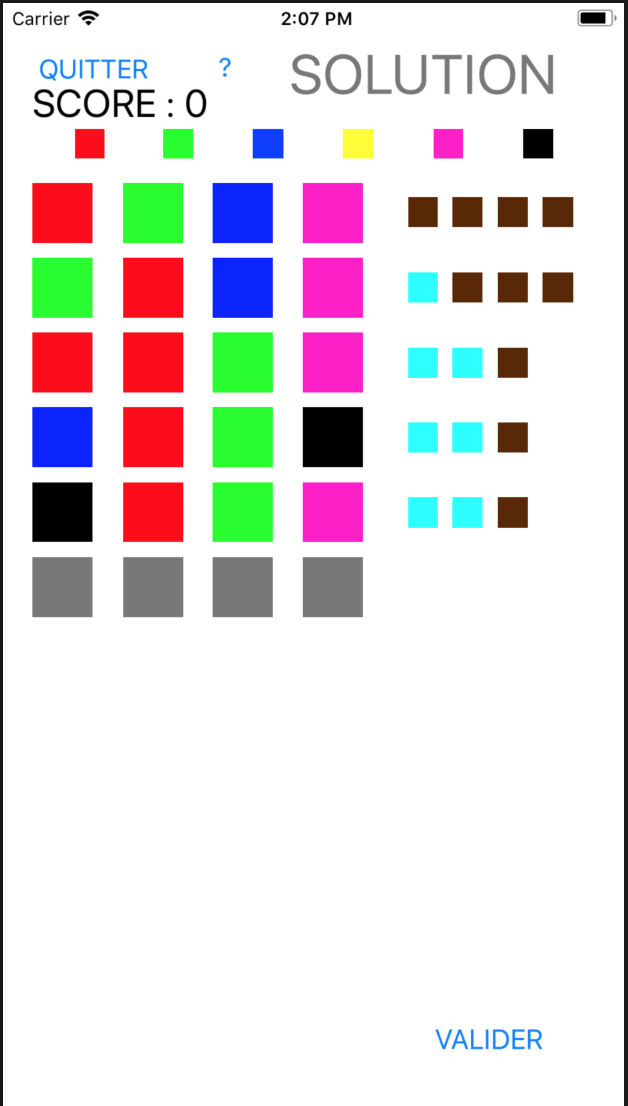
\includegraphics[scale = 0.3]{Interface}     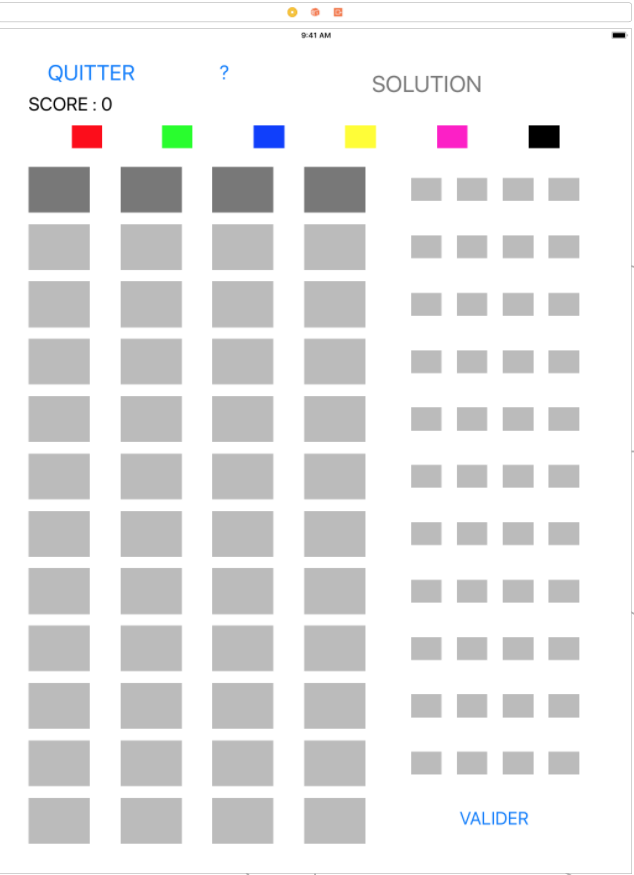
\includegraphics[scale = 0.4]{InterfaceB}
\end{center}
\indent A gauche on peut observer ce qu'aura l'utilisateur. ( iPhone 8 Plus ) 
 \\ A droite on peut observer ce que contient r\'{e}ellement l'application. ( iPad Pro 12.9" )

\section{Algorithmes}

Le jeu comporte peu de fonctions complexes. Nous en avons retenues deux : la validation d'un essai et l'aide apport\'{e}e \`{a} l'utilisateur \`{a} la suite de son essai. Nous pr\'{e}senteront ici les \'{e}v\'{e}nements composants la v\'{e}rification d'un essai et les cons\'{e}quences d'une bonne ou mauvaise r\'{e}ponse. 

\subsection{Validation}

\indent Les couleurs associ\'{e}es \`{a} l'essai sont compar\'{e}es avec celles qui composent la solution \`{a} la m\^{e}me place. Si l'essai et la combinaison \`{a} d\'{e}couvrir correspondent alors l'utilisateur obtiendra un nombre de points \'{e}gal \`{a} 12 - ( le nombre d'essais - 1 ). 
L'interface sera alors r\'{e}initialis\'{e}e, le score sera mis \`{a} jour et une nouvelle combinaison sera g\'{e}n\'{e}r\'{e}e.

\textit{Remarque} : L'utilisateur ne pourra pas valider une combinaison si elle ne comporte pas quatre couleurs.

\subsection{Bien plac\'{e}es et mal plac\'{e}es}
Afin de pouvoir aider le joueur dans le jeu voici comment est v\'{e}rifi\'{e} si l'emplacement d'une couleur est le bon si la couleur appartient \`{a} la solution. Dans notre jeu, le nombre de bonnes couleurs au bon endroit sera signal\'{e} par le m\^{e}me nombre de carr\'{e}s de couleur cyan. De m\^{e}me pour les bonnes couleurs au mauvais endroit avec une couleur marron.
Comme ci-dessous : 

\textit{Remarque : } La solution du jeu est affichée pour bien montrer que l'algorithme est juste.

\begin{center}
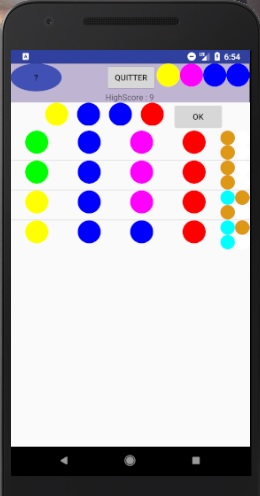
\includegraphics[scale = 0.5]{Ingame}
\end{center}
On d\'{e}finit ces valeurs en deux \'{e}tapes. Premi\`{e}rement on compare la couleur de chaque m\^{e}me emplacement entre l'essai et la solution. A chaque fois qu'on trouve une correspondance alors on augmente la variable qui contient le nombre de couleurs au bon endroit de 1. On marque alors les deux emplacement utilis\'{e}s \`{a} l'aide de deux listes. Puis on compare chaque couleur \`{a} toutes les autres couleurs. Si deux couleurs sont \'{e}gales, on v\'{e}rifie si ces deux couleurs n'ont pas d\'{e}j\`{a} \'{e}t\'{e} utilis\'{e}es. Si elles ne le sont pas alros on augmente la variable qui contient le nombre de couleurs au mauvais endroit de 1 puis on marque ces deux emplacements.

Soit le code commenté sous Android :
\begin{verbatim}
    public void check(int[] tab, int x) {
        boolean win = false;
        int indexx = x;
        nbbienplace = 0;
        nbmalplace = 0;
        int[] verifa = new int[4]; //tableau servant à marquer les couleurs déjà testées ou non pour la combinaison soluce
        int[] verifb = new int[4]; //pour la combinaison proposée

        //on test si on trouve les bonnes couleurs aux bons endroits
        for (int i = 0; i < 4; i++) {
            if (combi_soluce[i] == combinaison[i]) {
                nbbienplace++;
                indexx += 1;
                tab[indexx] = Color.CYAN;
                //on coche pour montrer que ces cercles sont déjà comparés et valides
                verifa[i] = 1;
                verifb[i] = 1;}
        }


        //on compare les cercles restants entre eux pour vérifier ceux qui sont mal placés
        for (int i = 0; i <= 3; i++) {
            for (int j = 0; j <= 3; j++) {
                //S'ils sont de la même couleurs et non marqués ils sont mal placés
                if ((combi_soluce[i] == combinaison[j]) && verifa[i] != 1 && verifb[j] != 1) {
                    nbmalplace++;
                    indexx += 1;
                    tab[indexx] = Color.rgb(223, 152, 20);
                    verifa[i] = 1;
                    verifb[j] = 1;}
            }
        }

        //Si tout est bien placé, le joueur a gagné
        if (nbbienplace == 4) {
            win();
            win = true;
        }

        //si le joueur dépasse 12 lignes, il a perdu
        if (nbrow >= 12 && !win) {
            lose();
        }
    }
\end{verbatim}

\section{Sauvegarde}
Une des contraintes que comportait ce projet \'{e}tait la possibilit\'{e} de pouvoir quitter une partie, de la sauvegarder puis de la reprendre ou la supprimer. La liste des parties sauvegard\'{e}es et la liste des scores devaient \^{e}tre pr\'{e}sent\'{e}es sous la forme de liste.

\subsection{Android}
Android possède plusieurs manières pour enregistrer les données de manière persistante. Nous avons choisi d'utiliser les SharedPreferences pour stocker toutes les informations nécessaires. 
Les ShraredPreference servent à stocker des informations grâce à un couple (valeur/clé). Les valeurs sont principalement de type simple (String, entier, booléen). Le seul type complexe géré dans les dernières versions d'Android sont les set. Ils permettent de stocker une liste de Strings.
\begin{verbatim}
SharedPreferences settings1 = getSharedPreferences("data", 0); //Créer/récupérer les sharedpreference du mot clé data
Set<String> set2 = settings1.getStringSet("data", null); //Récupérer les données
\end{verbatim}
Si le sharedPreference du mot clé data est null, alors set2 sera null.

Pour ce qui est de la présentation, nous avons choisi de faire confirmer la sauvegarde à l'utilisateur qui sera ensuite automatiquement redirigé vers l'écran des sauvegardes.
\begin{center}
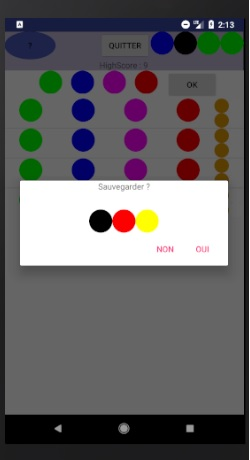
\includegraphics[scale = 0.5]{Popup_save}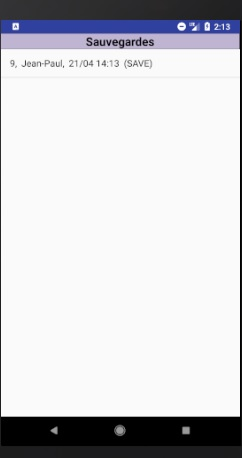
\includegraphics[scale = 0.5]{Saves}
\end{center}


\subsection{iOS}
Sous iOS, le syst\`{e}me de sauvegarde mis en place utilise \textit{UserDefaults.standard}. Nous avons donc d\'{e}clar\'{e} en variable globale une variable \textit{userData} que nous utiliserons pour stocker et extraire les diff\'{e}rentes valeurs n\'{e}cessaires \`{a} la partie de l'utilisateur telles que son score ou son nom. La d\'{e}claration et l'utilisation de cette variable se fait comme suit : 
\begin{verbatim}
let userData = UserDefaults.standard // Declaration
userData.set(0 , forKey: "s") // On stocke la valeur 0 avec comme clef "s"
s = userData.integer(forKey: "s") // On extrait la valeur avec comme clef "s" 
\end{verbatim}

\indent La sauvegarde n'est pas automatique. Elle se d\'{e}clenche lorsque l'utilisateur d\'{e}cide de quitter l'application en utilisant le bouton " QUITTER " et presse " OUI " \`{a} la demande d'enregistrement. Il lui sera alors propos\'{e} d'entrer son nom. L'utilisateur est oblig\'{e} d'entrer un nom pour enregistrer sa partie. Il pourra alors choisir l'un des trois emplacements disponibles.

\indent Lors de chaque sauvegarde on actualise la liste des trois scores les plus hauts atteints. M\^{e}me si le joueur perd, son score peut entrer dans ce classement si il est sup\'{e}rieur au score le plus bas du classement.

\indent Lorsque l'utilisateur perd une partie, il lui sera aussi proposer d'enregistrer sa partie. Il pourra donc cr\'{e}er sa propre sauvegarde mais recommencera avec un score \'{e}gal \`{a} 0.

\bigskip
\textit{Remarque} : A chaque sauvegarde est associ\'{e} le nom du joueur, son score ainsi que la date \`{a} laquelle la sauvegarde a \'{e}t\'{e} effectu\'{e}e. La liste des scores ne contiennent eux que le nom et le score du joueur.

\bigskip
\indent Afin de savoir \`{a} qui appartient la sauvegarde on utilise une variable globale \textit{MonIndex} qui contient le num\'{e}ro de la ligne sur laquelle l'utilisateur a appuy\'{e} lors du choix de la sauvegarde. On v\'{e}rifie donc toujours ce qu'elle contient afin de pouvoir sauvegarder correctement. 

\indent La sauvegarde est donc programm\'{e} de cette mani\`{e}re :

\begin{verbatim}
if(ChampTexte.text != ""){
            if ( monIndex == 0 ) {
                userData.set(ChampTexte.text,forKey: "n1")
                userData.set(dateDuJour(),forKey: "t1")
                userData.set(s,forKey: "s1")
                if(userData.integer(forKey: "s1")>=classement[2]){
                    classement[2] = userData.integer(forKey: "s1")
                    classement_nom[2] = userData.string(forKey: "n1")
                }
                if(perdu){ userData.set(0,forKey: "s1") }
            }
            ...
}
\end{verbatim}

\textit{Remarque} : Les variables \textit{classement} et \textit{classement\_nom} servent pour la sauvegarde des meilleurs scores ( nom et score du joueur ) 

\bigskip
\indent Pour ce qui est de la suppression de la sauvegarde, un choix est propos\'{e} au joueur quand il utilise le menu de sauvegarde. Il lui est demand\'{e} si il tient \`{a} charg\'{e} sa sauvegarde ou si il souhaite la supprimer. La suppression d'une sauvegarde remet \`{a} z\'{e}ro les valeurs des variables qui lui sont associ\'{e}es de la mani\`{e}re suivante : 

\begin{verbatim}
if(myIndex == 0){
	userData.set(0,forKey:"s1")
	userData.set(nil,forKey:"n1")
	userData.set("",forKey:"t1")
}
\end{verbatim}

\subsection{Problèmes rencontrés}
Dans notre cas, nous n'avons pas pu mettre en place un système 100\% fonctionnel de la sauvegarde sur les deux plateformes. En effet, dans le cas d'Android, il était assez difficile de sauvegarder l'intégralité des choix proposés par l'utilisateur ainsi que les indices de ces lignes dans un seul set. 
Il en était de même pour iOS qui demandait un nombre de ligne de code assez conséquentes sans possibilité de raccourcir.
Nous avons donc décidé de ne sauvegarder que les scores des parties choisies.


\section{Conclusion}

Globalement, nous avons pu respecter les règles imposées dans le CCTP, le jeu est fonctionnel, il y a un système de score complet avec classement ainsi que la possibilité de les supprimer. Seul le système de sauvegarde n'est pas optimal, mais nous avons pu arriver à un résultat fonctionnel sous forme de liste avec possibilité de suppression. 
Avec cet exercice complet, nous avons pu nous rendre compte de la force et des faiblesses des logiciels comme Android Studio et Xcode et de l'étendu des possibilités que l'on avait à portée de main pour développer sous téléphone.
Notre jeu a été une bonne expérience que l'on pourra toujours améliorer au fil du temps.

\section{Bibliographie}
\nocite{*} 
\bibliographystyle{plain}
\bibliography{ma_biblio}


\end{document}